\chapter{Theoretical basis}
\label{sec:theory}

\TODO{motivation and overview of chapter}

\section{Coordinate transformations}
\label{sec:theory:coord-transform}

A model implementation that uses terrain following layers must first choose from a variety of vertical coordinates.  The equations of motion with the hydrostatic approximation are simplified by using pressure coordinates \autocite{eliassen1949}.  However, because pressure varies in the horizontal, the lower boundary condition becomes complicated because surfaces of constant pressure intersect the terrain.  This motivated \textcite{phillips1957} to create the sigma coordinate in which pressure is normalised such that $\sigma$ ranges between zero at the top of the domain, and one at the surface.
Most hydrostatic models use normalised pressure coordinates.  With some exceptions, such as \textcite{xue-thorpe1991}, nonhydrostatic models use height-based coordinates \autocite{steppeler2003}.

Isentropic coordinates have also been investigated.  Since adiabatic motion follows isentropic surfaces, errors in discretising vertical advection are negligible.  However, difficulties arise when isentropes intersect with the surface \autocite{konor-arakawa1997}.

Second, a model may choose to use transformed coordinates.  Typically, terrain following models use transformed height or pressure coordinates so that the computational domain becomes rectangular.
Consider the two-dimensional cartesian coordinates $(x, z)$ and transformed coordinates $(x, \trans{z})$ which must be a monotonic function of $z$ so that the transformation is invertible.

A scalar field, $\varphi$, can be expressed in transformed coordinates as $\varphi(x, \trans{z})$ or in cartesian coordinates as $\varphi(x, \trans{z}(x, z))$.
Hence the vertical derivative of $\varphi$ can be found by using the chain rule \autocite{mit2004}
\begin{align}
  \frac{\partial \varphi}{\partial z} =
  \frac{\partial \varphi}{\partial \trans{z}}
  \frac{\partial \trans{z}}{\partial z} \label{eqn:theory:grad-transform}
\end{align}

The multivariable chain rule is needed to find the horizontal derivative.  Given a $m \times n$ Jacobi rotation matrix
\begin{align}
\frac{\partial y_i}{\partial x_k} = 
\begin{bmatrix}
  \dfrac{\partial y_1}{\partial x_1}	& \dfrac{\partial y_1}{\partial x_2} &	\cdots &	\dfrac{\partial y_1}{\partial x_n} \\
  \vdots				& \vdots &				\ddots &	\vdots \\
  \dfrac{\partial y_m}{\partial x_1}	& \dfrac{\partial y_m}{\partial x_2} &	\cdots &	\dfrac{\partial y_m}{\partial x_n}
\end{bmatrix}
%
\intertext{and similarly for $\partial y_i / \partial u_j$ and $\partial u_j / \partial x_k$ then we can express the chain rule as}
%
\frac{\partial y_i}{\partial x_k} = \frac{\partial y_i}{\partial u_j} \frac{\partial u_j}{\partial x_k}
%
\intertext{Applying this to $\varphi$ we find}
%
\begin{bmatrix}
	\frac{\partial \varphi}{\partial x}  &  \frac{\partial \varphi}{\partial z}
\end{bmatrix}
=
\begin{bmatrix}
	\frac{\partial \varphi}{\partial x}  &  \frac{\partial \varphi}{\partial \trans{z}}
\end{bmatrix}
\begin{bmatrix}
	\frac{\partial x}{\partial x} & 	\frac{\partial x}{\partial z} \\
	\frac{\partial \trans{z}}{\partial x} &	\frac{\partial \trans{z}}{\partial z}
\end{bmatrix} \label{eqn:theory:transform-matrix}
%
\intertext{and the horizontal component of equation~\ref{eqn:theory:transform-matrix} is then}
%
\left. \frac{\partial \varphi}{\partial x} \right|_z =
\left. \frac{\partial \varphi}{\partial x} \right|_\trans{z} +
	\frac{\partial \varphi}{\partial \trans{z}}
	\left. \frac{\partial \trans{z}}{\partial x} \right|_z \label{eq:theory:coord-trans}
\end{align}
where the subscript by the vertical bar denotes the variable that is held constant.

In a two-dimensional terrain-following coordinate transform, there is the added requirement that the transformed domain be rectangular.  This can be satisfied by imposing boundary conditions \autocite{schaer2002}
\begin{align}
	\trans{z}(x, \surface(x)) = 0 \quad,\quad \trans{z}(x, H) = H
\end{align}
where $H$ is the height of the domain and $h(x)$ is the height of the terrain surface.

\section{Horizontal pressure gradient}
In models that use TF coordinates, the horizontal pressure gradient can be calculated in the transformed coordinate system.  It follows from equation~\ref{eq:theory:coord-trans} that, in TF coordinates, the horizontal gradient of pressure $p$ is \autocite{mahrer1984}
\begin{align}
	\left. \frac{\partial p}{\partial x} \right|_z = 
	\left. \frac{\partial p}{\partial x} \right|_\trans{z} + 
	\left. \frac{\partial \trans{z}}{\partial x} \right|_z
	\frac{\partial p}{\partial \trans{z}} \label{eqn:theory:pressure-transform}
\end{align}
The first term on the right hand side is the change in pressure along the TF coordinate surface, and the second term corrects for the vertical variation in the first.  These terms tend to be large and of opposite sign over steep terrain, and a discretisation must be at least first order accurate so that the difference between the hydrostatic components of the two terms converges to zero \autocite{gary1973}.

\begin{figure}
	\centering
	\documentclass[tikz]{standalone}
\usepackage{bm}
\newcommand{\vect}{\bm}
\newcommand{\del}{\nabla}

\newcommand{\trans}[1]{{#1^\star}}
\newcommand{\surface}{h}
\newcommand{\shellcmd}[1]{\texttt{#1}}
\newcommand{\diffusioncoeff}{\mathcal{D}}
\newcommand{\exner}{\Pi}
\newcommand{\courant}{\mathrm{Co}}

\begin{document}
\begin{tikzpicture}[
  scale=0.5,
  cpnt/.style={fill=gray},
  arr/.style={thick, ->},
]
%\draw[gray, help lines] (0,0) grid (10,20);
\draw (0,0) -- (8,8) node[at end, anchor=south west] {$\trans{z}_{k-1}$};
\draw (0,8) -- (8,16) node[at end, anchor=south west] {$\trans{z}_k$};
\draw [dashed] (1,1) -- (1,9);
\draw [dashed] (7,7) -- (7,15);
\draw [dashed] (1,9) -- (7,9);
\path [cpnt] (1,1)  circle [radius=0.2] node[left] {$p_{i,k-1}$};
\path [cpnt] (1,9)  circle [radius=0.2] node[left] {$p_{i,k}$};
\path [cpnt] (7,7)  circle [radius=0.2] node[anchor=north west] {$p_{i+1,k-1}$};
\path [cpnt] (7,15) circle [radius=0.2] node[anchor=south east] {$p_{i+1,k}$};
\path [cpnt] (7,9) circle [radius=0.2] node[anchor=south east] {$p_{i+1,k-\Delta z}$};
\draw [<->] (1,8.6) -- (7,8.6) node[midway,below] {$\Delta x$};
\draw [<->] (7.4,9) -- (7.4,15) node[midway,right] {$\Delta z$};
\end{tikzpicture}
\end{document}

	\caption{Geometry of a first-order horizontal pressure gradient discretisation in a transformed coordinate.  Adapted from \textcite{mahrer1984}.}
	\label{fig:theory:pressure-error}
\end{figure}

A first-order forward difference approximation of a horizontal pressure gradient is shown in figure~\ref{fig:theory:pressure-error} where
\begin{align}
	\left. \frac{\partial p}{\partial x} \right|_z &= \frac{p_{i+1,k-\Delta z} - p_{i,k}}{\Delta x} + \mathcal{O}(\Delta x^2) \label{eqn:theory:p-grad}
%
	\intertext{where, in terrain following coordinates, the first term $p_{i+1,k-\Delta z}$ can be approximated by}
%
	p_{i+1,k-\Delta z} &= p_{i+1,j} - \left. \frac{\partial p}{\partial z} \right|_{i+1,j} \Delta z \label{eqn:theory:p-point} + \mathcal{O}(\Delta x^2)
%
	\intertext{Substituting equation~\ref{eqn:theory:p-point} into equation~\ref{eqn:theory:p-grad} we find}
%
	\left. \frac{\partial p}{\partial x} \right|_z &= \frac{p_{i+1,j} - p_{i,j}}{\Delta x} - \left. \frac{\Delta z}{\Delta x} \frac{\partial p}{\partial z} \right|_{i+1,j} \\
	&= \frac{p_{i+1,j} - p_{i,j}}{\Delta x} + \frac{\Delta z}{\Delta x} \frac{p_{i+1,j} - p_{i+1,j-1}}{z_j - z_{j-1}}
%
	\intertext{which, using equation~\ref{eqn:theory:grad-transform} to substitute $\trans{z}$ for $z$ becomes \textcite{mahrer1984}}
%
	\left. \frac{\partial p}{\partial x} \right|_z &= \frac{p_{i+1,j} - p_{i,j}}{\Delta x} + \frac{\partial \trans{z}}{\partial x} \frac{p_{i+1,j} - p_{i+1,j-1}}{\Delta \trans{z}}
\end{align}
which has the same form as equation~\ref{eqn:theory:pressure-transform}.
\TODO{how did the - become a +?}

Errors in the horizontal pressure gradient are associated with horizontal acceleration by the momentum equation, and have been shown to generate spurious winds \parencites{klemp2003}{klemp2011}.

Errors can be reduced by improving the accuracy of the horizontal pressure gradient discretisation.  \textcite{mahrer1984} proposed a discretisation where two pressure values at the same geometric height are interpolated from surrounding points.  From these values, a horizontal pressure gradient can be calculated without introducing metric terms.  Recent studies have found that variations of Mahrer's technique reduce spurious circulations \parencites{dempsey-davis1998}{klemp2011}{zaengl2012}.  \TODO{does this imply approach without metric terms is better than with?  can this be justified?}

\section{Terrain following techniques}
\label{sec:theory:tf}

\begin{figure}
	\captionsetup[subfigure]{position=b}
	\centering
	\subcaptionbox{Basic terrain following (BTF) \label{fig:intro:tf:btf}}[0.45\textwidth]{\input{btf-plot}}
	\hfill
	\subcaptionbox{Smooth level vertical (SLEVE) \label{fig:intro:tf:sleve}}[0.45\textwidth]{\input{sleve-plot}}
	\caption{Example vertical cross sections of terrain following layers illustrating the decay in terrain influence with height.   In BTF the decay is linear; in SLEVE it is exponential.}
	\label{fig:intro:tf}
\end{figure}

As well as improving discretisation accuracy, errors due to coordinate transformation can also be reduced by smoothing the effect of the terrain so that the grid becomes more regular aloft. 

\textcite{galchen-somerville1975} proposed a basic terrain following (BTF) coordinate system in which the terrain's influence decays linearly with height but disappears only at the top of the domain (example shown in figure~\ref{fig:intro:tf:btf}).  The transformation is defined as
\begin{align}
	\trans{z} &= H \frac{z - \surface}{H - \surface} \label{eqn:theory:btf}
%
\intertext{or}
%
	z &= \left( H - \surface \right) \frac{\trans{z}}{H} + \surface
\end{align}
where, in two dimensions, $z(x, \trans{z})$ is the height of the coordinate surface at level $\trans{z}$, $H$ is the height of the domain, and $\surface(x)$ is the height of the terrain surface.

The sigma coordinate transform of \textcite{phillips1957} is equivalent to the BTF coordinate transform since they both decay linearly.  However, since they decay with pressure rather than height, sigma coordinates also change with horizontal variations in pressure.

The hybrid terrain following (HTF) coordinates of \textcite{simmons-burridge1981} improve upon BTF coordinates by allowing the vertical decay profile can be controlled.  By choosing a suitable profile, terrain influence decays more rapidly than BTF to produce surfaces of constant height aloft \autocite{klemp2011}.

The coordinate system can be further refined by decaying small-scale features more rapidly than large-scale features to produce smooth coordinate surfaces in the middle and top of the domain.
\textcite{schaer2002} achieved with with smooth level vertical (SLEVE) coordinates in which terrain height is split into a large-scale component $\surface_1$ and a small-scale component $\surface_2$ such that $\surface = \surface_1 + \surface_2$.  Each component has a different exponential decay profile.  The transformation is defined as
\begin{align}
	z &= \trans{z} + \surface_1 b_1 + \surface_2 b_2
%
\intertext{with the vertical decay functions are given by}
%
	b_i &= \frac{\sinh \left( \left( H - \trans{z} \right) / s_i \right)}{\sinh \left( H / s_i \right)}
\end{align}
where $s_1$ and $s_2$ are the scale heights of large-scale and small-scale terrain respectively.  SLEVE produces smooth coordinate surfaces in the middle and top of the domain (see figure~\ref{fig:intro:tf:sleve}).

\textcite{leuenberger2010} generalised the SLEVE transformation in order to increase cell thickness in the layers nearest the ground, allowing longer timesteps and permitting more accurate calculation of parameterised low-level heat and momentum fluxes.  An exponent $n$ is introduced so that the generalised decay functions become
\begin{align}
	b_i &= \frac{\sinh \left( \left( H / s_i \right)^n - \left( \trans{z} / s_i \right)^n \right)}{\sinh \left( H / s_i \right)^n}
\end{align}
where the optimal exponent value was found to be $n = 1.35$.

In the smoothed terrain following (STF) coordinate, \textcite{klemp2011} took an alternative approach, using a multipass smoothing operator, and found that errors were reduced still further compared to SLEVE.


\section{Cell shaving techniques}
\label{sec:theory:shaving}

\begin{figure}
	\captionsetup[subfigure]{position=b}
	\centering
	\subcaptionbox{Full-step \label{fig:intro:shaved:full}}[0.32\textwidth]{\input{full-step-plot}}
	\subcaptionbox{Partial-step \label{fig:intro:shaved:partial}}[0.32\textwidth]{\input{partial-step-plot}}
	\subcaptionbox{Piecewise linear.  Grid boxes marked with asterisk ($\ast$) denote small cells. \label{fig:intro:shaved:piecewise-linear}}[0.32\textwidth]{\input{cut-cell-plot}}
	\caption{Vertical cross sections illustrating different methods of shaving cells intersecting with a hypothetical surface (heavy line).  Adapted from \textcite{adcroft1997}.}
	\label{fig:intro:shaved}
\end{figure}

\textcite{mesinger1988} proposed a grid that, like terrain following grids, retains almost-constant cell sizes.  The step-mountain (or `full-step') coordinate removes cells that are intersected by the terrain so creating steps over the surface (see figure~\ref{fig:intro:shaved:full}).  \textcite{gallus-klemp2000} found that lee slope winds are too weak over smooth orography, but this study did not examine performance over steep terrain.  In contrast, \textcite{mesinger2004} compared results from three operational NCEP models that suggested the step-coordinate model was more skillful than the TF coordinate models in forecasting precipitation over the mountainous western United States.

\textcite{adcroft1997} proposed a partial-step system for modelling the ocean surface in which the cell height is adjusted so that cell volume is accurately represented (figure~\ref{fig:intro:shaved:partial}).  Compared to the full-step approach of \textcite{mesinger1988}, spurious oscillations were significantly reduced advecting a tracer over topography.

The piecewise linear cut cell method is another alternative to terrain following layers.  Here, the surface terrain is intersected with a regular cartesian grid such that cells are cut where they intersect with the ground (see figure~\ref{fig:intro:shaved:piecewise-linear}).  
This leads to cells that are entirely above the surface, entirely below it, and those which intersect with the ground.  Those cells which intersect the ground have, in two dimensions, a triangular, trapezoidal or pentagonal shape \autocite{rosatti2005}.  Figure~\ref{fig:intro:shaved:piecewise-linear} shows an example of this method.  In some grid boxes, small cells, marked with an asterisk ($\ast$), are created by intersection with the surface.
The primary difficulty is with numerical stability and reduced model efficiency associated with small cells. \TODOsidenote{also, vertical resolution varies at mountain top, leads to only 1st order accuracy for 2nd order schemes... need to find citation}

A variety of solutions to the `small cell problem' have been proposed.  In \textcite{yamazaki-satomura2010}, small cells are combined with horizontally or vertically adjacent cells.  \textcite{steppeler2002} use a `thin-wall' approximation to increase the computational volume of small cells without altering the terrain.  Conceptually, each cell partially or completely below the mountain is filled with air and surrounded by a thin wall.  Where a cell is cut by the terrain, the computational volume is equal to that of an uncut cell.  \textcite{jebens2011} avoid the timestep restriction associated with explicit schemes by using an implicit method for cut cells and a semi-explicit method elsewhere.


\section{Finite volume method}
\label{sec:theory:fv}

The finite volume method is a discretisation technique that represents the spatial domain as a grid of cells.  A volumetric scalar field $\varphi$ is then discretised by modelling the average value in each cell located at its centre.  At each timestep, cell averages are updated by considering the flux $\vect{F}$ across the faces of the cell surface.  In atmospheric modelling, $\vect{F}$ is typically the advective flux $\vect{u} \varphi$ where $\vect{u}$ is the velocity field.

The notation used in this project for the representation discrete variables follows \textcite{weller-shahrokhi2014}.  A cell average of $\varphi$ is written as $\varphi_c$, where $c$ denotes a cell.  A volumetric vector field $\psi$ located at a face is written as $\psi_f$, where $f$ denotes a cell face.  An interpolation of cell centre averages of $\varphi$ onto a face $f$ is written as $\varphi_F$.  $f \in \: c$ represents the faces of a cell.  $c \in \: f$ represents the cells $c$ that share a face $f$.

To develop the finite volume method, we start by considering the conservation of $\varphi$
\begin{align}
	\frac{\partial \varphi}{\partial t} + \del \cdot \left( \vect{u} \varphi \right) = 0
%
\intertext{Taking the volume integral over a cell $c$ with volume $V_c$ we find}
%
	\int_{V_c} \frac{\partial \varphi}{\partial t} \diff V + \int_{V_c} \del \cdot \left( \vect{u} \varphi \right) \diff V &= 0
%
\intertext{Integrating the first term gives the cell average $\varphi_c$ and applying the divergence theorem to the second term gives a surface integral, hence}
%
	V_c \frac{\partial \varphi_c}{\partial t} + \int_{S_c} \varphi \vect{u} \cdot \nunit \diff S &= 0
%
\intertext{where $S_c$ is the cell surface area and $\nunit$ is the unit vector that is outward normal to the surface.  Dividing by the cell volume and, for a cell with a finite number of surfaces, this becomes}
%
	\frac{\partial \varphi_c}{\partial t} + \frac{1}{V_c} \sum_{f \in \: c} \varphi_F \vect{u}_f \cdot \nunit S_f &= 0 \label{eqn:theory:discrete-continuity}
\end{align}
where $S_f$ is the surface area of face $f$, and $\varphi_F$ is the interpolated value of $\varphi$ at the face.  This interpolation of cell averages onto faces is a significant source of truncation error in finite volume systems \autocite{adcroft1997}.

The finite volume method leads to a staggering of variables with fluxes at cell faces similar to an Arakawa C grid.  Because cell averages are modified only through surface fluxes, a quantity of $\varphi$ the fluxes out of one cell must flux into another.  Thus, $\varphi$ is conserved in the finite volume method.

\section{Vertical staggering of variables}
\label{sec:theory:staggering}

\TODO{if this section is staying in Theory chapter, make sure you define variables here and you can skip some of them in Discretisation of Euler equations later on}

\begin{figure}
	\centering
	\documentclass[tikz]{standalone}
\usepackage{bm}
\usetikzlibrary{patterns}
\newcommand{\vect}{\bm}
\newcommand{\del}{\nabla}

\newcommand{\trans}[1]{{#1^\star}}
\newcommand{\surface}{h}
\newcommand{\shellcmd}[1]{\texttt{#1}}
\newcommand{\diffusioncoeff}{\mathcal{D}}
\newcommand{\exner}{\Pi}
\newcommand{\courant}{\mathrm{Co}}

\begin{document}
\begin{tikzpicture}[
  scale=0.7
]
\fill [pattern=north west lines] (0,0) rectangle (6,-0.4);
\fill [pattern=north west lines] (8,0) rectangle (14,-0.4);
\node at (7,0) {$\frac{1}{2}$};
\draw [dashed] (0,0) -- (6,0) node [at start, anchor=east] {$w$};
\draw [dashed] (8,0) -- (14,0) node [at end, anchor=west] {$\theta, w$};

\node at (7,1) {$1$};
\draw (0,1) -- (6,1) node [at start, anchor=east] {$u, v, \theta, \rho, \exner$};
\draw (8,1) -- (14,1) node [at end, anchor=west] {$u, v, \rho, \exner$};

\node at (7,2) {$\frac{3}{2}$};
\draw [dashed] (0,2) -- (6,2) node [at start, anchor=east] {$w$};
\draw [dashed] (8,2) -- (14,2) node [at end, anchor=west] {$\theta, w$};

\node at (7,3) {$2$};
\draw (0,3) -- (6,3) node [at start, anchor=east] {$u, v, \theta, \rho, \exner$};
\draw (8,3) -- (14,3) node [at end, anchor=west] {$u, v, \rho, \exner$};

\node at (7,4) {$\frac{5}{2}$};
\draw [dashed] (0,4) -- (6,4) node [at start, anchor=east] {$w$};
\draw [dashed] (8,4) -- (14,4) node [at end, anchor=west] {$\theta, w$};

\node at (3,5) {$\vdots$};
\node at (11,5) {$\vdots$};

\node at (7,6) {$k - \frac{1}{2}$};
\draw [dashed] (0,6) -- (6,6) node [at start, anchor=east] {$w$};
\draw [dashed] (8,6) -- (14,6) node [at end, anchor=west] {$\theta, w$};

\node at (7,7) {$k$};
\draw (0,7) -- (6,7) node [at start, anchor=east] {$u, v, \theta, \rho, \exner$};
\draw (8,7) -- (14,7) node [at end, anchor=west] {$u, v, \rho, \exner$};

\node at (7,8) {$k + \frac{1}{2}$};
\draw [dashed] (0,8) -- (6,8) node [at start, anchor=east] {$w$};
\draw [dashed] (8,8) -- (14,8) node [at end, anchor=west] {$\theta, w$};

\node at (7,9) {$k + 1$};
\draw (0,9) -- (6,9) node [at start, anchor=east] {$u, v, \theta, \rho, \exner$};
\draw (8,9) -- (14,9) node [at end, anchor=west] {$u, v, \rho, \exner$};

\node at (7,10) {$k + \frac{3}{2}$};
\draw [dashed] (0,10) -- (6,10) node [at start, anchor=east] {$w$};
\draw [dashed] (8,10) -- (14,10) node [at end, anchor=west] {$\theta, w$};

\node at (3,11) {$\vdots$};
\node at (11,11) {$\vdots$};
\end{tikzpicture}
\end{document}

	\caption{Lorenz (left) and Charney--Phillips (right) vertical staggering of variables.  Solid lines represent full levels, dashed lines represent half levels.  Adapted from \textcite{holdaway2013}.}
	\label{fig:theory:staggering}
\end{figure}

When discretising the equations of motion, computational properties including stability and convergence are necessary.  Additionally, it is desirable to obtain a discretisation that represents the dynamics of the real system.  There are two commonly-used vertical staggerings, the Lorenz grid \autocite{lorenz1960} and the Charney--Phillips grid \autocite{charney-phillips1953}, which offer different sets of computational and physical mimetic properties.

In both grids, horizontal velocities $u$ and $v$, and density $\rho$, are stored at full levels.  Mass flux is computed with the vertical velocity $w$ at half levels.  The two grids differ in their placement of potential temperature, $\theta$: on the Charney--Phillips grid it is stored at half levels, and at full levels on the Lorenz grid.  These arrangements of variables are summarised in figure~\ref{fig:theory:staggering}.

The Charney--Philips grid was originally developed for a quasigeostrophic model using sigma coordinates.  \textcite{arakawa-moorthi1988} found that advection of quasi-geostrophic potential vorticity is conserved by this grid staggering, and it requires less interpolation of variables than the Lorenz grid \autocite{holdaway2013}. \TODO{anything else of significant interest to say about it?}

The Lorenz grid has a number of mimetic properties: it conserves total energy, the mean potential temperature, and variance of potential temperature assuming no diabatic processes or friction \autocite{arakawa-konor1996}.  However, it is known that a computational mode exists on the Lorenz grid which can create a zig-zag in the vertical distribution of potential temperature \parencites{arakawa-moorthi1988}{arakawa-konor1996}{holdaway2013b}.  This can be explained by considering the vertical momentum equation \autocite{holdaway2013}
\begin{align}
	\frac{\partial w}{\partial t} + \vect{u} \cdot \del w = -g - c_p \theta \frac{\partial \exner}{\partial z}
\end{align}
In a discretisation of this equation, to calculate $w_{k+\frac{1}{2}}$, $\theta_{k+\frac{1}{2}}$ may be interpolated using an arithmetic mean of the adjacent values $\theta_k$ and $\theta_{k+1}$.  As shown in figure~\ref{fig:theory:theta-oscillation}, a grid-scale vertical wave in potential temperature would not be visible by the model \autocite{holdaway2013}.  \TODO{I hope I've got this right.  I can't find very detailed information so I've plugged the gaps myself.}

The computational mode can affect the physical mode, causing spurious interactions with condensation processes \autocite{arakawa-konor1996} and the spurious generation of baroclinic instability and increased gravity wave activity \parencites{arakawa-moorthi1988}{cullen1997}.

\begin{figure}
	\centering
	\documentclass[tikz]{standalone}
\usepackage{bm}
\usetikzlibrary{patterns}
\newcommand{\vect}{\bm}
\newcommand{\del}{\nabla}

\newcommand{\trans}[1]{{#1^\star}}
\newcommand{\surface}{h}
\newcommand{\shellcmd}[1]{\texttt{#1}}
\newcommand{\diffusioncoeff}{\mathcal{D}}
\newcommand{\exner}{\Pi}
\newcommand{\courant}{\mathrm{Co}}

\begin{document}
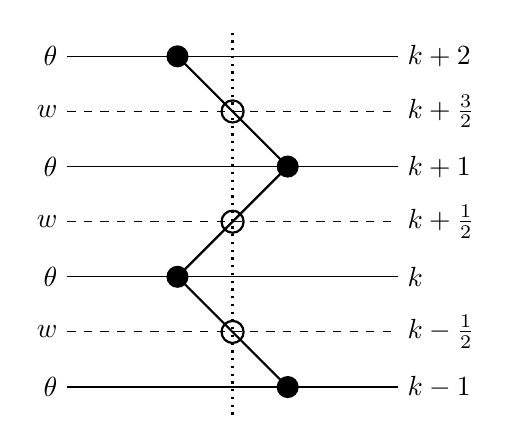
\begin{tikzpicture}[
  scale=0.7,
  cpnt/.style={fill=black}
]
\draw (0,0) -- (6,0) node [at start, anchor=east] {$\theta$} node [at end, anchor=west] {$k-1$};
\draw [dashed] (0,1) -- (6,1) node [at start, anchor=east] {$w$} node [at end, anchor=west] {$k-\frac{1}{2}$};
\draw (0,2) -- (6,2) node [at start, anchor=east] {$\theta$} node [at end, anchor=west] {$k$};
\draw [dashed] (0,3) -- (6,3) node [at start, anchor=east] {$w$} node [at end, anchor=west] {$k+\frac{1}{2}$};
\draw (0,4) -- (6,4) node [at start, anchor=east] {$\theta$} node [at end, anchor=west] {$k+1$};
\draw [dashed] (0,5) -- (6,5) node [at start, anchor=east] {$w$} node [at end, anchor=west] {$k+\frac{3}{2}$};
\draw (0,6) -- (6,6) node [at start, anchor=east] {$\theta$} node [at end, anchor=west] {$k+2$};

\path [cpnt] (4,0) circle [radius=0.2];
\path [cpnt] (2,2) circle [radius=0.2];
\path [cpnt] (4,4) circle [radius=0.2];
\path [cpnt] (2,6) circle [radius=0.2];
\draw [thick] (3,1) circle [radius=0.2];
\draw [thick] (3,3) circle [radius=0.2];
\draw [thick] (3,5) circle [radius=0.2];

\draw [thick] (4,0) -- (2,2) -- (4,4) -- (2,6);
\draw [thick, dotted] (3,-0.5) -- (3,6.5);
\end{tikzpicture}
\end{document}

	\caption{Interpolation of potential temperature on a Lorenz grid.  Solid circles denote values of $\theta$ stored at full levels and the solid line shows the potential temperature profile.  Open circles denote $\theta$ values interpolated onto half levels and the dotted line represents the interpolated profile.  Magnitude of $\theta$ increases to the right.}
	\label{fig:theory:theta-oscillation}
\end{figure}

\section{Gravity waves}
\label{sec:theory:gw}

When an air parcel is forced to rise over a mountain, it experiences a restoring buoyancy force which can create waves that propagate away from the mountain.  These are known as gravity waves, mountain waves, or lee waves.

\TODO{create lenticular clouds, clear air turbulence, strong downslope winds (Holton 2003)}

Two dimensional waves in the $x-z$ plane are characterised by their horizontal and vertical wavenumbers, $k$ and $m$, their frequency, $\omega$, and amplitude $\amplitude$.  By starting with the Boussinesq approximation of the Navier-Stokes equations we can derive the dispersion relation \autocite{lynch-cassano2006}
\begin{align}
	\left( \frac{\partial}{\partial t} + \overline{u} \frac{\partial}{\partial x} \right)^2
	\left( \frac{\partial^2 w'}{\partial x^2} + \frac{\partial^2 w'}{\partial z^2} \right) +
	N^2 \frac{\partial^2 w'}{\partial x^2} = 0
%
	\intertext{where $\overline{u}$ is the mean horizontal wind and $w'$ is the vertical velocity anomaly.  This can be solved by assuming a wave-like solution}
%
	w' = \amplitude \cos \left( kx + mz - \omega t \right) \label{eqn:theory:gw:w-prime}
	\intertext{thus giving the dispersion relation}
	\left( \omega - \overline{u}k \right)^2 
	\left( k^2 + m^2 \right) -
	N^2 k^2 = 0
\end{align}

The potential temperature anomaly $\theta'$ is a function of background stability $\partial \overline{\theta}/\partial z$ and is \ang{90} out of phase with $w'$, given by \autocite{lynch-cassano2006} \TODO{it'd be nice to derive this from Boussinesq equations but I've struggled to do it myself}
\begin{align}
	\theta' &= \frac{\amplitude}{\omega} \frac{\diff{\overline{\theta}}}{\diff{z}} \sin \phase \label{eqn:theory:gw:theta-prime}
%
	\intertext{where the phase $\phase$ is}
%
	\phase &= kx + mz - \omega t \label{eqn:theory:gw:phase}
\end{align}

\begin{figure}
	\centering
	\documentclass[tikz]{standalone}
\usepackage{bm}
\usetikzlibrary{arrows}
\newcommand{\vect}{\bm}
\newcommand{\del}{\nabla}

\newcommand{\trans}[1]{{#1^\star}}
\newcommand{\surface}{h}
\newcommand{\shellcmd}[1]{\texttt{#1}}
\newcommand{\diffusioncoeff}{\mathcal{D}}
\newcommand{\exner}{\Pi}
\newcommand{\courant}{\mathrm{Co}}

\begin{document}
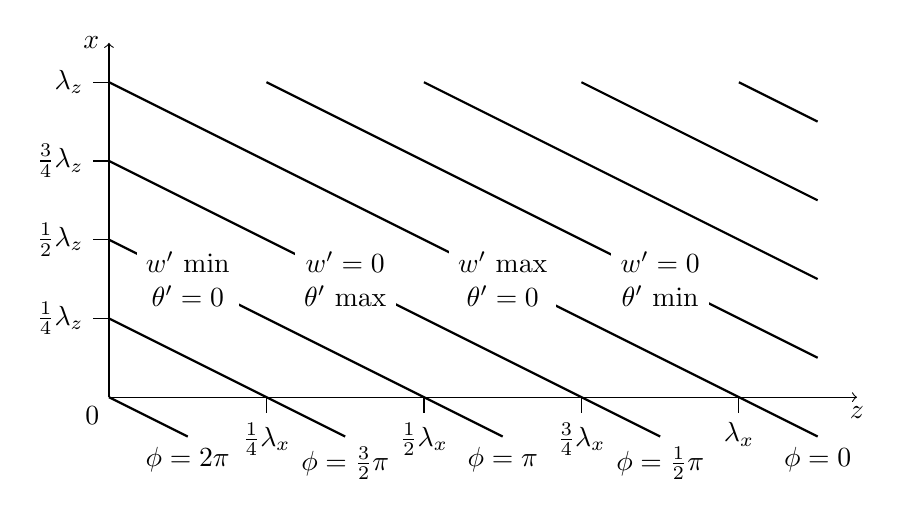
\begin{tikzpicture}[
  cpnt/.style={fill=gray},
  arr/.style={thick, ->},
]
\draw [->] (0,0) -- (0,4.5) node [at end, anchor=east] {$x$} node [at start, anchor=north east] {$0$};
\draw [->] (0,0) -- (9.5,0) node [at end, anchor=north] {$z$};

\draw [thick] (0,0) -- (1,-0.5) node [at end, anchor=north] {$\phi = 2 \pi$};
\draw [thick] (0,1) -- (3,-0.5) node [at end, anchor=north] {$\phi = \frac{3}{2} \pi$};
\draw [thick] (0,2) -- (5,-0.5) node [at end, anchor=north] {$\phi = \pi$};
\draw [thick] (0,3) -- (7,-0.5) node [at end, anchor=north] {$\phi = \frac{1}{2} \pi$};
\draw [thick] (0,4) -- (9,-0.5) node [at end, anchor=north] {$\phi = 0$};
\draw [thick] (2,4) -- (9,0.5);
\draw [thick] (4,4) -- (9,1.5);
\draw [thick] (6,4) -- (9,2.5);
\draw [thick] (8,4) -- (9,3.5);

\node [fill=white, align=center] at (1,1.5) {$w'$ min\\$\theta' = 0$};
\node [fill=white, align=center] at (3,1.5) {$w' = 0$\\$\theta'$ max};
\node [fill=white, align=center] at (5,1.5) {$w'$ max\\$\theta' = 0$};
\node [fill=white, align=center] at (7,1.5) {$w' = 0$\\$\theta'$ min};

\draw (0,1) -- (-0.2,1) node [at end, anchor=east] {$\frac{1}{4} \lambda_z$};
\draw (0,2) -- (-0.2,2) node [at end, anchor=east] {$\frac{1}{2} \lambda_z$};
\draw (0,3) -- (-0.2,3) node [at end, anchor=east] {$\frac{3}{4} \lambda_z$};
\draw (0,4) -- (-0.2,4) node [at end, anchor=east] {$\lambda_z$};

\draw (2,0) -- (2,-0.2) node [at end, anchor=north] {$\frac{1}{4} \lambda_x$};
\draw (4,0) -- (4,-0.2) node [at end, anchor=north] {$\frac{1}{2} \lambda_x$};
\draw (6,0) -- (6,-0.2) node [at end, anchor=north] {$\frac{3}{4} \lambda_x$};
\draw (8,0) -- (8,-0.2) node [at end, anchor=north] {$\lambda_x$};

\end{tikzpicture}
\end{document}

	\caption{Phase relationship between vertical velocity anomalies $w'$ and potential temperature anomalies $\theta'$.  Adapted from \textcite{lynch-cassano2006}.}
	\label{fig:theory:gw:phases}
\end{figure}

Using equations~\ref{eqn:theory:gw:w-prime}, \ref{eqn:theory:gw:theta-prime} and \ref{eqn:theory:gw:phase} we can plot the phase relationships between $w'$ and $\theta'$, shown in figure~\ref{fig:theory:gw:phases}.

\TODO{discuss infinite sinusoidal hill, then finite hill by sum of infinite sine waves, as in Lynch\&Cassano}


\begin{align}
	h(x) &= h_0 \cos \left( kx \right) \\
	w &= \frac{\diff{h}}{\diff{t}}
	w &= \overline{u} \frac{\partial h}{\partial x} \\
	w &= - \overline{u} k h_0 \sin \left( kx \right)
\end{align}

\TODO{$|\overline{u}k| < N$ when widely spaced ridges have small wavenumber $k$, propagate vertically.  also, weak wind or strong stability satisfy the condition.  Conversely, evanescent wave created when ridge is narrow, large wavenumber $k$ (or large windspeed or weak stability).}
